\chapter{Methodology}\label{chapter:Methodology}
This chapter proposes an algorithm, which is capable to overcome the restrictions of the ortho algorithm reviewed as state of the art in chapter \ref{chapter:SotA}. Therefore three different signal distribution networks are introduced. Namely an input, a majority and a sequential network. The name signal distribution networks comes from the resulting algorithm, which still lays combinational logic in the same fashion as the original ortho algorithm and only makes changes to the clocking scheme, when implementing irregular parts. Thus, distributing signals in a way that the new functionality can be implemented within the placement and routing procedure used by ortho. Further, because the 2DD-Wave scheme is used for the ortho algorithm, every majority gate and sequential circuit is seen as an irregularity or rather a signal distribution network that is put into the regular ortho scheme. In the following first the input network is discussed, which aims to reduce area in the input region of the layout. Afterwards the networks used for implementing majority gates and sequential parts are discussed and analyzed.

\section{Input Network}
Looking again at the resulting layout of a 2:1 mux or ortho in \ref{fig:ortho_mux_21}, it can be seen that in the rows where inputs are placed, no other gates are put, because the space is used for rewiring in order to solve conflicts. The idea of the input network is to allow gates also to be placed in this area to save space and also place inputs in a way that wire crossings may be minimized. Recalling the pseudo-code from the ortho algorithm, an input has a conflict when it is colored south because it is not allowed to wire over the other inputs laying in the same column. This means the area overhead in the input region is highly dependent on the coloring assigned to the outgoing edges of the inputs. The algorithm used in the pseudo-code in $3$ is implemented in a way that just finds \textit{some} valid coloring for the given logic network. Unfortunately due to the algorithms nature it often assigns the color south to exactly these edges resulting in the said area overhead. One approach to solve this problem is to improve the coloring of the logic network and prevent excess wiring. Secondly a new rule for edges colored south inside the conflicting area can be introduced, making the rewiring redundant. The third idea, which can be implemented in the input network is an ordering of the inputs in order to allow those who are connected with the same gates to be placed near each other in order to reduce wire expenses and crossings.

\begin{algorithm}[H]
	\vdots
	
	\begin{algorithmic}
		\State Convert $N$ to a 3-graph by substitution and balance inverters at fan-out nodes
		\State Order primary input nodes
		\State \vdots
		\State Generate \textbf{conditional} direction assignment $d : \Delta \rightarrow \{east, south\}$ and subdivide signals if necessary
		\State Compute topological ordering $v_1, . . . , v_i \in N$
		\State Extend $L$ by one column and reserve it for primary inputs
		\ForAll {vertex $v_1, ..., v_i \in N $ with at most two incoming signals $\sigma_1, \sigma_2$}
		\If{vertex $v$ is terminal/primary input}
		\State Extend $L$ by one row
		\State Place v at position $(0, h - 1)$
		\ElsIf{$d(\sigma_1) = d(\sigma_2) = east$}
		\State \vdots
		\ElsIf { signals are labeled $south$}
		\If{\textbf{not} root node exists}
		\State Extend $L$ by one row
		\EndIf
		\State $w_p \leftarrow$ max. horizontal position of v's predecessors
		\State Place v at position $(w _p, h - 1)$
		\EndIf
		
		\EndFor
		\State \vdots \\
		\Return $L$
	\end{algorithmic}
	\caption{Ortho changes with input network}\label{alg:input_network}
\end{algorithm}

To discuss the idea, first the parts of the logic network and the layout are part of the input network. If we look at the layout again the input network describes mostly the rows in which the inputs are placed, and whose area should be utilized. The viewed parts of the logic network are all primary inputs and the gates which they are wired to, skipping over inverters. This means that if the outgoing edge of an primary input is an inverter, the gate hanging on the outgoing edge of the inverter is considered. Starting with the different gates inputs can be connected to, the coloring they can have should be discussed. One-input nodes including inverters and fan-out nodes can be all wired east due to the fact that the primary input they are connected to only have one outgoing edge. This means that the coloring can be selected arbitrarily because no dependencies exist and in this case always the non-conflicting $east$ assignment is chosen. When looking at two-input logic gates like AND and OR gates it has to be seen that the coloring can only be chosen arbitrarily if both input nodes are primary inputs. In every other case the direction assignment has to consider the coloring of the other incoming edge of the gate. Thus, first every primary input connected to a fan-out node and the fan-out node itself should be placed into the layout. This has several reasons. First of all the fan-out nodes give the constraints for the conditional coloring which is introduced in the input network. Also fan-out nodes produce excess wiring, which means that they should be connected to their outgoing gates as fast as possible. With the fan-out gates placed into the network we can now see that every fan-out gate needs exactly one output assigned with color $east$ and one output assigned with color $south$. Considering that the gate connected to the edge colored $south$ demands also his second incoming edge to be colored $south$ and the second incoming edge could be connected to a primary input, we can see that a conditional coloring alone is not powerful enough to resolve all conflicts. For this case the coloring $south$ is allowed in order to preserve the direction assignment rules but a new placement rule is introduced. The original algorithm part (line 14-22) handling the placement of nodes based on their coloring makes sure that every gate placed $east$ occupies a new column and every node colored $south$ occupies a new row. Considering now the case of a $south$ coloring a new rule can be deduced for a special case. If a node is labeled south and its predecessor, which has the lower horizontal position \textbf{also} has the higher vertical position, it is called the \textit{root node} and the layout isn't extended by a column but the gate is still placed to position $w_p, h-1$. Following this rule the gate is now placed in the same column as its predecessor with the higher y-coordinate. If we apply this to a two-input gate in the input network with a primary input and a fan-out node as predecessors, the primary input is always the root node due to the ordering and new coloring. Thus, the new rule allows the two-input gate connected to the $south$ colored primary input and the fan-out node to be placed in the same column as the primary input, resulting in no conflict because the node is not \textit{actually} placed southern of its predecessors. It was found that this rule could not only be utilized of this special case but also for the general $south$ placement in the algorithm with one exception. Looking at fan-out nodes and considering a fan-out node to be the root node, the coloring would wire both the eastern and the southern colored outgoing edges onto the same row, which is not allowed here. The resulting pseudo-code snippets replacing the used code are shown in !!. Also it has to be considered that this coloring still needs to include helping nodes e.g. when three fan-out nodes are connected to each other. Preceding to the coloring, the input nodes need to be ordered according to the ideas presented. Thus, primary input nodes connected to fan-out nodes are placed first. Then the primary input nodes, which are connected to the outgoing edges of the fan-out nodes are placed. This is done to reduce the distance between coherent gates and therefore also the number of wire crossings. Afterwards primary inputs directly connected to a gate which has its other incoming edge connected to a second primary input are placed. Finally all input nodes, which are not connected to the rest of the input network are placed arbitrarily.
Some other issues are related to inverter nodes. As already mentioned they are skipped in the view of the input network. Considering an inverter node which is assigned $south$ e.g. after a fan-out node and it should be placed in the same row as an primary input, again a conflict arises because the input cannot wire to the east. Thus, all inverters colored $south$ need to be placed to minimum the row of the most southern primary input plus one, in order to prevent to much overhead produced by inverters also a balancing network is introduced. Based on the substitution of the logic network into $N$ with inverter and fan-out nodes it can happen that a fan-out node has two inverters connected to its outgoing edges. In this case these inverters are substituted again by one single inverter as incoming node to the fan-out, resulting in an overall lower number of inverter nodes.

\begin{figure}
	\centering
	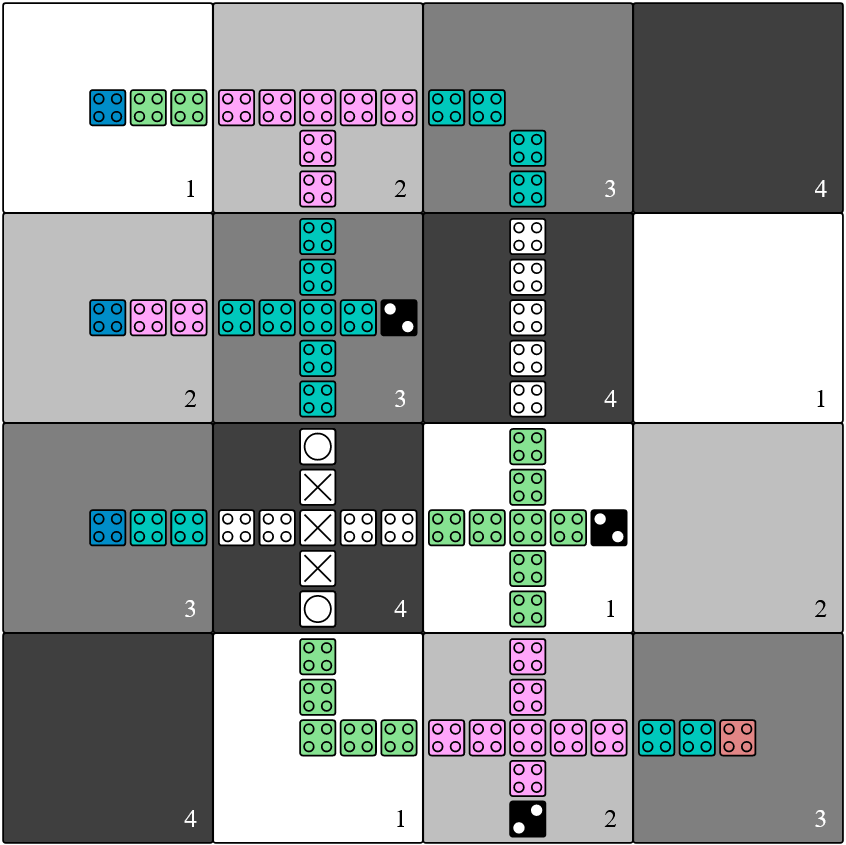
\includegraphics[scale=0.5]{input_network_mux_21}
	\caption{Placement and routing of a 2:1 mux network using the ortho algorithm with the input network}\label{fig:input_network_mux_21}
\end{figure}

Figure \ref{fig:input_network_mux_21} shows the placement and routing of the ortho algorithm after implementing the proposed input network. It can be quickly seen that the resulting layout saves up place and even wire crossings. The ordering of the inputs puts first the fan-out node and then the two connected primary inputs. In this case the input network also considered the inverter at the outgoing edge to be colored east in order to produce less overhead, because if the inverter would be colored $south$ it would have to be placed underneath the primary inputs. Looking at the AND gate connecting the fan-out with the second primary input, we can see that the new rule for nodes placed south is used. This also applies for the AND gate connecting the third primary output to the inverter. The last OR gate is placed after the normal rules of the ortho algorithm. The exact results are shown in the next chapter.

\section{Majority Gates Placement Network}
Reference to the importance of this part in the QCA technology. \\
Point out that 2DD-Wave is still used but clocking scheme is adjusted to place majority gates.\\
This is why buffers have to be used.\\
Point out the overhead that is produced by buffers.\\
Maybe assumption why it doesn't make sense to only use RES. (you lose really much space for the cells which are no majority gates)


\section{Sequential Circuits Placement}

Importance of sequential circuits.\\
Point out how the registers are implemented.\\
Show how the distribution network is generated, where Ris and Ros are placed and how they are treated within the network.\\
Make clear that this implementation is slowing down the circuit significantly.